\documentclass{standalone}
\usepackage{tikz}

\begin{document}
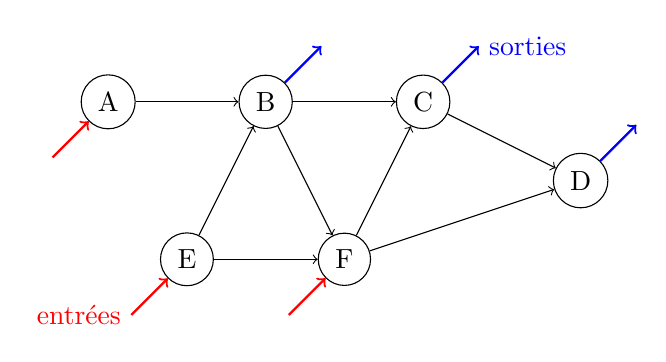
\begin{tikzpicture}

\node [circle, draw] (A) at (0, 0) {A};
\node [circle, draw] (B) at (2, 0) {B};
\node [circle, draw] (C) at (4, 0) {C};
\node [circle, draw] (D) at (6, -1) {D};
\node [circle, draw] (E) at (1, -2) {E};
\node [circle, draw] (F) at (3, -2) {F};

\draw[->] (A) -- (B);
\draw[->] (B) -- (C);
\draw[->] (C) -- (D);
\draw[->] (E) -- (F);
\draw[->] (F) -- (D);
\draw[->] (E) -- (B);
\draw[->] (B) -- (F);
\draw[->] (F) -- (C);

\draw[thick, <-, red] (A) -- ++ (225:1);
\draw[thick, <-, red] (E) -- ++ (225:1) node[left] {entrées};
\draw[thick, <-, red] (F) -- ++ (225:1);

\draw[thick, ->, blue] (B) -- ++ (45:1);
\draw[thick, ->, blue] (C) -- ++ (45:1) node[right] {sorties};
\draw[thick, ->, blue] (D) -- ++ (45:1);

\end{tikzpicture}
\end{document}